% answers.tex —— 2002 年·春季上海卷 · 参考答案与详细解析片段
% 由 tools/generate_projects.py 依来源总账自 2002/2002_数学真题_春季上海_试题.md + 2002/2002_数学真题_春季上海_解析正文.md + 2002/2002_数学真题_春季上海_答案要点.md 生成，勿手改（改源 MD 后重跑）


\begin{gktip}
固定源 PDF 为印刷页码 99–100 的两页题面，不附答案。以下解析均依据题面独立复算；第 10、11、12、19 题的图形在 LaTeX 工程中以 TikZ/PGFPlots 矢量源重绘。
\end{gktip}

\gkpart{一、填空题}

\begin{answer}
\gksolhead{1}{}

\textbf{题目}：

\Needspace{5\baselineskip}
函数

\nopagebreak[4]
\[
y=\frac1{3-2x-x^2}
\]

的定义域为\gkblank{}。

\Needspace{4\baselineskip}
\textbf{解析}

\Needspace{5\baselineskip}
分母不能为零。由

\nopagebreak[4]
\[
3-2x-x^2=0
\Longleftrightarrow
(x-1)(x+3)=0
\]

\Needspace{5\baselineskip}
得 $x=1$ 或 $x=-3$。所以定义域为

\nopagebreak[4]
\[
\mathbb R\setminus\{-3,1\}.
\]

\gkanswer{答案：$\mathbb R\setminus\{-3,1\}$。}

\end{answer}
\begin{answer}
\gksolhead{2}{}

\textbf{题目}：

若椭圆的两个焦点坐标为 $F_1(-1,0)$、$F_2(5,0)$，长轴长为 $10$，则椭圆的方程为\gkblank{}。

\Needspace{4\baselineskip}
\textbf{解析}

\Needspace{5\baselineskip}
椭圆中心为两个焦点的中点 $(2,0)$，焦半距 $c=3$。长轴长为 $10$，所以 $a=5$，从而

\nopagebreak[4]
\[
b^2=a^2-c^2=25-9=16.
\]

\Needspace{5\baselineskip}
故椭圆方程为

\nopagebreak[4]
\[
\frac{(x-2)^2}{25}+\frac{y^2}{16}=1.
\]

\gkanswer{答案：$\dfrac{(x-2)^2}{25}+\dfrac{y^2}{16}=1$。}

\end{answer}
\begin{answer}
\gksolhead{3}{}

\textbf{题目}：

\Needspace{5\baselineskip}
若全集 $I=\mathbb R$，$f(x)\text{、}g(x)$ 均为 $x$ 的二次函数，

\nopagebreak[4]
\[
P=\{x\mid f(x)<0\},\qquad Q=\{x\mid g(x)\ge0\}
\]

\Needspace{5\baselineskip}
则不等式组

\nopagebreak[4]
\[
\begin{cases}
f(x)<0,\\
g(x)<0
\end{cases}
\]

的解集可用 $P\text{、}Q$ 表示为\gkblank{}。

\Needspace{4\baselineskip}
\textbf{解析}

\Needspace{5\baselineskip}
$f(x)<0$ 的解集是 $P$。由于 $Q$ 表示 $g(x)\ge0$ 的解集，$g(x)<0$ 的解集就是 $Q$ 在全集 $\mathbb R$ 中的补集 $Q^c$。因此所求解集为

\nopagebreak[4]
\[
P\cap Q^c.
\]

\gkanswer{答案：$P\cap Q^c$。}

\end{answer}
\begin{answer}
\gksolhead{4}{}

\textbf{题目}：

设 $f(x)$ 是定义在 $\mathbb R$ 上的奇函数。若当 $x\ge0$ 时，$f(x)=\log_3(1+x)$，则 $f(-2)=$\gkblank{}。

\Needspace{4\baselineskip}
\textbf{解析}

\Needspace{5\baselineskip}
由奇函数性质，

\nopagebreak[4]
\[
f(-2)=-f(2)=-\log_3(1+2)=-1.
\]

\gkanswer{答案：$-1$。}

\end{answer}
\begin{answer}
\gksolhead{5}{}

\textbf{题目}：

\Needspace{5\baselineskip}
若在

\nopagebreak[4]
\[
\left(\sqrt[5]{x}-\frac1x\right)^n
\]

的展开式中，第 $4$ 项是常数项，则 $n=$\gkblank{}。

\Needspace{4\baselineskip}
\textbf{解析}

\Needspace{5\baselineskip}
展开式的第 $4$ 项对应从第二项中取出 $3$ 个因子，因此其 $x$ 的幂为

\nopagebreak[4]
\[
\left(x^{1/5}\right)^{n-3}\left(x^{-1}\right)^3
=x^{(n-18)/5}.
\]

\Needspace{5\baselineskip}
第 $4$ 项为常数项，故

\nopagebreak[4]
\[
\frac{n-18}{5}=0,
\qquad n=18.
\]

\gkanswer{答案：$18$。}

\end{answer}
\begin{answer}
\gksolhead{6}{}

\textbf{题目}：

\Needspace{5\baselineskip}
已知

\nopagebreak[4]
\[
f(x)=\sqrt{\frac{1-x}{1+x}}
\]

若 $\alpha\in\left(\frac\pi2,\pi\right)$，则 $f(\cos\alpha)+f(-\cos\alpha)$ 可化简为\gkblank{}。

\Needspace{4\baselineskip}
\textbf{解析}

\Needspace{5\baselineskip}
利用半角公式以及 $\alpha/2\in(\pi/4,\pi/2)$，有

\nopagebreak[4]
\[
f(\cos\alpha)
=\sqrt{\frac{1-\cos\alpha}{1+\cos\alpha}}
=\tan\frac\alpha2,
\]

\nopagebreak[4]
\[
f(-\cos\alpha)
=\sqrt{\frac{1+\cos\alpha}{1-\cos\alpha}}
=\cot\frac\alpha2.
\]

\Needspace{5\baselineskip}
所以

\nopagebreak[4]
\[
f(\cos\alpha)+f(-\cos\alpha)
=\tan\frac\alpha2+\cot\frac\alpha2
=\frac{2}{\sin\alpha}.
\]

\gkanswer{答案：$\dfrac2{\sin\alpha}$。}

\end{answer}
\begin{answer}
\gksolhead{7}{}

\textbf{题目}：

六位身高全不相同的同学拍照留念，摄影师要求前后两排各三人，

则后排每人均比前排同学高的概率是\gkblank{}。

\Needspace{4\baselineskip}
\textbf{解析}

\Needspace{5\baselineskip}
把前后两排按位置配成三个对应位置。对每一对位置，较高者在后排、较矮者在前排的概率为 $1/2$。三对位置的高矮方向在随机排列下等可能，因此所求概率为

\nopagebreak[4]
\[
\left(\frac12\right)^3=\frac18.
\]

\gkanswer{答案：$\dfrac18$。}

\end{answer}
\begin{answer}
\gksolhead{8}{}

\textbf{题目}：

设曲线 $C_1$ 和 $C_2$ 的方程分别为 $F_1(x,y)=0$ 和 $F_2(x,y)=0$，则点 $P(a,b)\notin C_1\cap C_2$ 的一个充分条件为\gkblank{}。

\Needspace{4\baselineskip}
\textbf{解析}

\Needspace{5\baselineskip}
若点 $P(a,b)$ 同时属于两条曲线，则必有 $F_1(a,b)=0$ 且 $F_2(a,b)=0$。因此只要其中一个等式不成立，就足以保证该点不在交集内。例如条件

\nopagebreak[4]
\[
F_1(a,b)\ne0\quad\text{\text{或}}\quad F_2(a,b)\ne0
\]

就是一个充分条件。

\gkanswer{答案：$F_1(a,b)\ne0$ 或 $F_2(a,b)\ne0$。}

\end{answer}
\begin{answer}
\gksolhead{9}{}

\textbf{题目}：

\Needspace{5\baselineskip}
若 $f(x)=2\sin\omega x$（$0<\omega<1$）在区间

\nopagebreak[4]
\[
\left[0,\frac\pi3\right]
\]

上的最大值是 $\sqrt2$，则 $\omega=$\gkblank{}。

\Needspace{4\baselineskip}
\textbf{解析}

\Needspace{5\baselineskip}
因为 $0<\omega<1$，所以当 $x\in[0,\pi/3]$ 时，

\nopagebreak[4]
\[
0\le\omega x\le\frac\pi3<\frac\pi2.
\]

\Needspace{5\baselineskip}
$\sin(\omega x)$ 在该区间上递增，最大值在 $x=\pi/3$ 处取得。因此

\nopagebreak[4]
\[
2\sin\frac{\omega\pi}{3}=\sqrt2.
\]

\Needspace{5\baselineskip}
又 $\omega\pi/3\in(0,\pi/3)$，故 $\omega\pi/3=\pi/4$，从而

\nopagebreak[4]
\[
\omega=\frac34.
\]

\gkanswer{答案：$\dfrac34$。}

\end{answer}
\begin{answer}
\gksolhead{10}{}

\textbf{题目}：

如图表示一个正方体表面的一种展开图，图中的四条线段 $AB\text{、}CD\text{、}EF$ 和 $GH$ 在原正方体中相互异面的有\gkblank{}对。
\nopagebreak[4]
\begin{center}% 2002 年春季上海卷第 10 题：正方体展开图
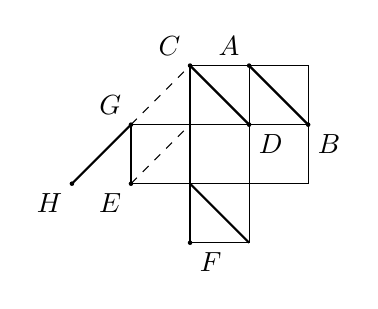
\begin{tikzpicture}[scale=0.75]
  \draw (0,0) rectangle (1,1);
  \draw (1,0) rectangle (2,1);
  \draw (2,0) rectangle (3,1);
  \draw (1,1) rectangle (2,2);
  \draw (2,1) rectangle (3,2);
  \draw (1,-1) rectangle (2,0);

  \draw[thick] (-1,0)--(0,1);
  \draw[thick] (1,2)--(2,1);
  \draw[thick] (2,2)--(3,1);
  \draw[thick] (1,0)--(2,-1);

  \draw[dashed] (0,1)--(1,2) (0,0)--(1,1);

  \fill (-1,0) circle (1.1pt) node[below left] {$H$};
  \fill (0,1) circle (1.1pt) node[above left] {$G$};
  \fill (0,0) circle (1.1pt) node[below left] {$E$};
  \fill (1,-1) circle (1.1pt) node[below right] {$F$};
  \fill (1,2) circle (1.1pt) node[above left] {$C$};
  \fill (2,1) circle (1.1pt) node[below right] {$D$};
  \fill (2,2) circle (1.1pt) node[above left] {$A$};
  \fill (3,1) circle (1.1pt) node[below right] {$B$};
\end{tikzpicture}
\end{center}
\nopagebreak[4]
\Needspace{4\baselineskip}
\textbf{解析}

\Needspace{5\baselineskip}
将展开图的六个正方形折回同一正方体后，逐一比较四条线段所在的棱及其方向。相互异面的线段对为

\nopagebreak[4]
\[
EF\text{ \text{与} }HG,\qquad AB\text{ \text{与} }HG,\qquad AB\text{ \text{与} }CD.
\]

因此共有 $3$ 对。

\gkanswer{答案：$3$ 对。相互异面的线段对可记为 $EF$ 与 $HG$、$AB$ 与 $HG$、$AB$ 与 $CD$。}

\end{answer}
\begin{answer}
\gksolhead{11}{}

\textbf{题目}：

如图所示，客轮以速度 $2v$ 由 $A$ 至 $B$ 再到 $C$ 匀速航行，货轮从 $AC$ 的中点 $D$ 出发，以速度 $v$ 沿直线匀速航行，将货物送达客轮。已知 $AB\perp BC$，且 $AB=BC=50$ 海里。若两船同时出发，则两船相遇之处距 $C$ 点\gkblank{}海里。（结果精确到小数点后 $1$ 位）
\nopagebreak[4]
\begin{center}% 2002 年春季上海卷第 11 题：客轮与货轮航线
\begin{tikzpicture}[>=stealth, scale=0.85]
  \coordinate (A) at (0,0);
  \coordinate (B) at (3.2,0);
  \coordinate (C) at (3.2,2.5);
  \coordinate (D) at (1.6,1.25);

  \draw[thick] (A)--(B)--(C);
  \draw[dashed] (A)--(C);
  \fill (A) circle (1.1pt) node[below left] {$A$};
  \fill (B) circle (1.1pt) node[below right] {$B$};
  \fill (C) circle (1.1pt) node[above right] {$C$};
  \fill (D) circle (1.1pt) node[left] {$D$};
\end{tikzpicture}
\end{center}
\nopagebreak[4]
\Needspace{4\baselineskip}
\textbf{解析}

\Needspace{5\baselineskip}
取坐标

\nopagebreak[4]
\[
A=(0,0),\quad B=(50,0),\quad C=(50,50),\quad D=(25,25).
\]

\Needspace{5\baselineskip}
客轮先沿 $AB$ 行驶。若相遇点在 $AB$ 上，记其横坐标为 $x$，由同时到达条件有

\nopagebreak[4]
\[
\sqrt{(x-25)^2+25^2}=\frac{x}{2}.
\]

\Needspace{5\baselineskip}
这会导出

\nopagebreak[4]
\[
3x^2-200x+5000=0,
\]

其判别式为负，所以相遇点不在 $AB$ 上，只能在 $BC$ 上。

\Needspace{5\baselineskip}
设相遇点为 $M=(50,y)$，其中 $0\le y\le50$。客轮从 $A$ 到 $M$ 的路程为 $50+y$，故用时为 $(50+y)/(2v)$；货轮行驶距离为

\nopagebreak[4]
\[
DM=\sqrt{25^2+(y-25)^2},
\]

\Needspace{5\baselineskip}
用时为 $DM/v$。令两者相等并平方，得

\nopagebreak[4]
\[
25^2+(y-25)^2=\left(\frac{50+y}{2}\right)^2,
\]

\Needspace{5\baselineskip}
即

\nopagebreak[4]
\[
3y^2-300y+2500=0.
\]

\Needspace{5\baselineskip}
在 $[0,50]$ 内的根为

\nopagebreak[4]
\[
y=50-\frac{50\sqrt6}{3}.
\]

\Needspace{5\baselineskip}
所以相遇点距 $C$ 的距离为

\nopagebreak[4]
\[
50-y=\frac{50\sqrt6}{3}\approx40.8.
\]

\gkanswer{答案：$\dfrac{50\sqrt6}{3}\text{ \text{海里}}\approx40.8\text{ \text{海里}}$。}

\end{answer}
\begin{answer}
\gksolhead{12}{}

\textbf{题目}：

\Needspace{5\baselineskip}
如图，若从点 $O$ 所作的两条射线 $OM\text{、}ON$ 上分别有点 $M_1\text{、}M_2$ 与点 $N_1\text{、}N_2$，则

\nopagebreak[4]
\[
\frac{S_{\triangle OM_1N_1}}{S_{\triangle OM_2N_2}}
=\frac{OM_1}{OM_2}\cdot\frac{ON_1}{ON_2}
\]

若从点 $O$ 所作的不在同一平面内的三条射线 $OP\text{、}OQ\text{、}OR$ 上，分别有点 $P_1\text{、}P_2$，点 $Q_1\text{、}Q_2$ 和点 $R_1\text{、}R_2$，则类似的结论为\gkblank{}。
\nopagebreak[4]
\begin{center}% 2002 年春季上海卷第 12 题：平面三角形与空间三棱锥比例
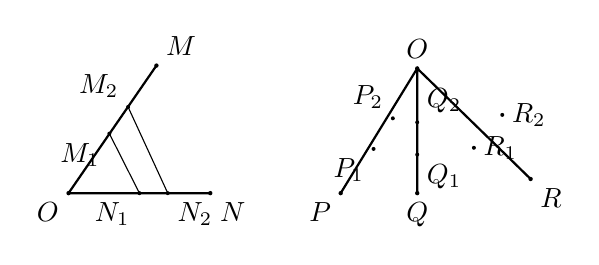
\begin{tikzpicture}[>=stealth, scale=0.72]
  % 两条共面射线
  \begin{scope}
    \coordinate (O) at (0,0);
    \coordinate (M) at (1.55,2.25);
    \coordinate (N) at (2.5,0);
    \coordinate (Mone) at (0.72,1.05);
    \coordinate (Mtwo) at (1.05,1.52);
    \coordinate (None) at (1.25,0);
    \coordinate (Ntwo) at (1.75,0);
    \draw[thick] (O)--(M) (O)--(N);
    \draw (Mone)--(None) (Mtwo)--(Ntwo);
    \fill (O) circle (1.1pt) node[below left] {$O$};
    \fill (M) circle (1.1pt) node[above right] {$M$};
    \fill (N) circle (1.1pt) node[below right] {$N$};
    \fill (Mone) circle (1.0pt) node[below left] {$M_1$};
    \fill (Mtwo) circle (1.0pt) node[above left] {$M_2$};
    \fill (None) circle (1.0pt) node[below left] {$N_1$};
    \fill (Ntwo) circle (1.0pt) node[below right] {$N_2$};
  \end{scope}

  % 三条不共面射线的透视示意
  \begin{scope}[xshift=4.8cm]
    \coordinate (Otwo) at (1.35,2.2);
    \coordinate (P) at (0,0);
    \coordinate (Q) at (1.35,0);
    \coordinate (R) at (3.35,0.25);
    \draw[thick] (Otwo)--(P) (Otwo)--(Q) (Otwo)--(R);
    \coordinate (Pone) at (0.58,0.78);
    \coordinate (Ptwo) at (0.92,1.32);
    \coordinate (Qone) at (1.35,0.68);
    \coordinate (Qtwo) at (1.35,1.25);
    \coordinate (Rone) at (2.35,0.80);
    \coordinate (Rtwo) at (2.85,1.38);
    \fill (Otwo) circle (1.1pt) node[above] {$O$};
    \fill (P) circle (1.1pt) node[below left] {$P$};
    \fill (Q) circle (1.1pt) node[below] {$Q$};
    \fill (R) circle (1.1pt) node[below right] {$R$};
    \fill (Pone) circle (1.0pt) node[below left] {$P_1$};
    \fill (Ptwo) circle (1.0pt) node[above left] {$P_2$};
    \fill (Qone) circle (1.0pt) node[below right] {$Q_1$};
    \fill (Qtwo) circle (1.0pt) node[above right] {$Q_2$};
    \fill (Rone) circle (1.0pt) node[right] {$R_1$};
    \fill (Rtwo) circle (1.0pt) node[right] {$R_2$};
  \end{scope}
\end{tikzpicture}
\end{center}
\nopagebreak[4]
\Needspace{4\baselineskip}
\textbf{解析}

\Needspace{5\baselineskip}
以 $O$ 为公共顶点的三棱锥体积可表示为

\nopagebreak[4]
\[
V=\frac16\left|\det(\overrightarrow{OP},\overrightarrow{OQ},\overrightarrow{OR})\right|.
\]

\Needspace{5\baselineskip}
同一条射线上的向量只发生长度倍乘，所以行列式的三列分别按三个比例因子变化。因此

\nopagebreak[4]
\[
\frac{V_{OP_1Q_1R_1}}{V_{OP_2Q_2R_2}}
=\frac{OP_1}{OP_2}\cdot\frac{OQ_1}{OQ_2}\cdot\frac{OR_1}{OR_2}.
\]

\gkanswer{答案：$\displaystyle\frac{V_{OP_1Q_1R_1}}{V_{OP_2Q_2R_2}}=\frac{OP_1}{OP_2}\cdot\frac{OQ_1}{OQ_2}\cdot\frac{OR_1}{OR_2}$。}

\end{answer}
\gkpart{二、选择题}

\begin{answer}
\gksolhead{13}{}

\textbf{题目}：

若 $a\text{、}b\text{、}c$ 为任意向量，$m\in\mathbb R$，则下列等式不一定成立的是\mbox{（　　）}

（A）$(a+b)+c=a+(b+c)$　　（B）$(a+b)\cdot c=a\cdot c+b\cdot c$

（C）$m(a+b)=ma+mb$　　（D）$(a\cdot b)c=a(b\cdot c)$

\Needspace{4\baselineskip}
\textbf{解析}

向量加法满足结合律，数量乘法对向量加法满足分配律，点积也满足对向量加法的分配律。一般情况下，向量 $(a\cdot b)c$ 与 $a(b\cdot c)$ 并不相等，例如取三个互相垂直的非零向量即可。因此选 D。

\gkanswer{答案：D。}

\end{answer}
\begin{answer}
\gksolhead{14}{}

\textbf{题目}：

在 $\triangle ABC$ 中，若 $2\cos B\sin A=\sin C$，则 $\triangle ABC$ 的形状一定是\mbox{（　　）}

（A）等腰直角三角形　　（B）直角三角形　　（C）等腰三角形　　（D）等边三角形

\Needspace{4\baselineskip}
\textbf{解析}

\Needspace{5\baselineskip}
由 $C=\pi-A-B$，

\nopagebreak[4]
\[
\sin C=\sin(A+B)=\sin A\cos B+\cos A\sin B.
\]

\Needspace{5\baselineskip}
代入已知条件得

\nopagebreak[4]
\[
\sin A\cos B=\cos A\sin B,
\]

即 $\sin(A-B)=0$。由于 $A\text{、}B\in(0,\pi)$ 且 $A+B<\pi$，只能有 $A=B$。所以三角形为等腰三角形，选 C。

\gkanswer{答案：C。}

\end{answer}
\begin{answer}
\gksolhead{15}{}

\textbf{题目}：

设 $A>0$，$a\ne1$，函数 $y=\log_a x$ 的反函数和 $y=\log_a\dfrac1x$ 的反函数的图象关于\mbox{（　　）}

（A）$x$ 轴对称　　（B）$y$ 轴对称　　（C）$y=x$ 对称　　（D）原点对称

\Needspace{4\baselineskip}
\textbf{解析}

\Needspace{5\baselineskip}
$y=\log_a x$ 的反函数为 $y=a^x$。由

\nopagebreak[4]
\[
y=\log_a\frac1x
\Longleftrightarrow
x=a^{-y},
\]

其反函数为 $y=a^{-x}$。图象 $y=a^x$ 与 $y=a^{-x}$ 互为关于 $y$ 轴的对称图形，选 B。

\gkanswer{答案：B。}

\end{answer}
\begin{answer}
\gksolhead{16}{}

\textbf{题目}：

设 $\{a_n\}$（$n\in\mathbb N$）是等差数列，$S_n$ 是其前 $n$ 项的和，且 $S_5<S_6$，$S_6=S_7>S_8$，则下列结论错误的是\mbox{（　　）}

（A）$d<0$　　（B）$a_7=0$　　（C）$S_9>S_5$　　（D）$S_6$ 和 $S_7$ 均为 $S_n$ 的最大值

\Needspace{4\baselineskip}
\textbf{解析}

由 $S_6=S_7$ 得 $a_7=0$。又 $S_5<S_6$ 得 $a_6>0$，所以公差 $d=a_7-a_6<0$。于是 $a_1,\ldots,a_6>0$，而 $a_8,a_9<0$，故 $S_6=S_7$ 是最大值。

\Needspace{5\baselineskip}
此外

\nopagebreak[4]
\[
S_9-S_5=a_6+a_7+a_8+a_9
=(-d)+0+d+2d=2d<0,
\]

所以 $S_9<S_5$，选项 C 错误。

\gkanswer{答案：C。}

\end{answer}
\gkpart{三、解答题}

\begin{answer}
\gksolhead{17}{}

\textbf{题目}：

\Needspace{5\baselineskip}
已知 $z\text{、}\omega$ 为复数，$(1+3i)z$ 为纯虚数，

\nopagebreak[4]
\[
\omega=\frac z{2+i}
\]

且 $|\omega|=5\sqrt2$，求 $\omega$。

\Needspace{4\baselineskip}
\textbf{解析}

\Needspace{5\baselineskip}
设 $z=x+yi$。由 $(1+3i)z$ 为纯虚数，其实部为零，故

\nopagebreak[4]
\[
x-3y=0.
\]

\Needspace{5\baselineskip}
所以可设 $z=t(3+i)$，其中 $t\in\mathbb R$。于是

\nopagebreak[4]
\[
\omega=\frac{t(3+i)}{2+i}
=\frac{t(3+i)(2-i)}5
=\frac t5(7-i).
\]

\Needspace{5\baselineskip}
由 $|\omega|=5\sqrt2$ 得

\nopagebreak[4]
\[
\frac{|t|}{5}\sqrt{50}=5\sqrt2,
\qquad |t|=5.
\]

\Needspace{5\baselineskip}
故

\nopagebreak[4]
\[
\omega=7-i\quad\text{\text{或}}\quad\omega=-7+i.
\]

\gkanswer{答案：$\omega=7-i$ 或 $\omega=-7+i$。}

\end{answer}
\begin{answer}
\gksolhead{18}{}

\textbf{题目}：

\Needspace{5\baselineskip}
已知 $F_1\text{、}F_2$ 为双曲线

\nopagebreak[4]
\[
\frac{x^2}{a^2}-\frac{y^2}{b^2}=1\qquad(a>0,\ b>0)
\]

的焦点。过 $F_2$ 作垂直 $x$ 轴的直线交双曲线于点 $P$，且 $\angle PF_1F_2=30^\circ$，求双曲线的渐近方程。

\Needspace{4\baselineskip}
\textbf{解析}

\Needspace{5\baselineskip}
设焦半距为 $c$，则 $c^2=a^2+b^2$，焦点为 $F_1(-c,0)$、$F_2(c,0)$。过 $F_2$ 的竖线与双曲线交于 $P$，故

\nopagebreak[4]
\[
|y_P|=\frac{b^2}{a}.
\]

\Needspace{5\baselineskip}
在直角坐标中，$\overrightarrow{F_1F_2}$ 为水平向量，故由 $\angle PF_1F_2=30^\circ$，

\nopagebreak[4]
\[
\tan30^\circ=\frac{b^2/a}{2c},
\qquad
\frac{b^2}{a}=\frac{2c}{\sqrt3}.
\]

\Needspace{5\baselineskip}
令 $r=b^2/a^2$，代入 $c=a\sqrt{1+r}$，得

\nopagebreak[4]
\[
r=\frac2{\sqrt3}\sqrt{1+r}.
\]

\Needspace{5\baselineskip}
平方并取正根：

\nopagebreak[4]
\[
3r^2=4(1+r)
\Longrightarrow
3r^2-4r-4=0
\Longrightarrow r=2.
\]

\Needspace{5\baselineskip}
所以 $b^2=2a^2$，双曲线的渐近线为

\nopagebreak[4]
\[
y=\pm\frac ba x=\pm\sqrt2\,x.
\]

\gkanswer{答案：$y=\pm\sqrt2x$。}

\end{answer}
\begin{answer}
\gksolhead{19}{}

\textbf{题目}：

如图，三棱柱 $OAB-O_1A_1B_1$，平面 $OBB_1O_1\perp$ 平面 $OAB$，$\angle O_1OB=60^\circ$，$\angle AOB=90^\circ$，且 $OB=OO_1=2$，$OA=\sqrt3$。求：
\nopagebreak[4]
\begin{center}% 2002 年春季上海卷第 19 题：三棱柱空间图形
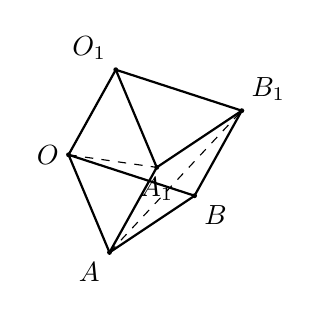
\begin{tikzpicture}[>=stealth, scale=0.8]
  \coordinate (O) at (0,0);
  \coordinate (B) at (2.0,-0.65);
  \coordinate (A) at (0.65,-1.55);
  \coordinate (Oone) at (0.75,1.35);
  \coordinate (Bone) at (2.75,0.70);
  \coordinate (Aone) at (1.4,-0.20);

  \draw[thick] (O)--(B)--(A)--cycle;
  \draw[thick] (Oone)--(Bone)--(Aone)--cycle;
  \draw[thick] (O)--(Oone) (B)--(Bone) (A)--(Aone);
  \draw[dashed] (O)--(Aone) (A)--(Bone);

  \fill (O) circle (1.1pt) node[left] {$O$};
  \fill (B) circle (1.1pt) node[below right] {$B$};
  \fill (A) circle (1.1pt) node[below left] {$A$};
  \fill (Oone) circle (1.1pt) node[above left] {$O_1$};
  \fill (Bone) circle (1.1pt) node[above right] {$B_1$};
  \fill (Aone) circle (1.1pt) node[below] {$A_1$};
\end{tikzpicture}
\end{center}
\nopagebreak[4]
（1） 二面角 $O_1-AB-O$ 的大小；

（2） 异面直线 $A_1B$ 与 $AO_1$ 所成角的大小。

（上述结果用反三角函数值表示）

\Needspace{4\baselineskip}
\textbf{解析}

\Needspace{5\baselineskip}
建立空间直角坐标系，取

\nopagebreak[4]
\[
O=(0,0,0),\quad B=(2,0,0),\quad A=(0,\sqrt3,0).
\]

\Needspace{5\baselineskip}
由 $OO_1=2$、$\angle O_1OB=60^\circ$ 以及棱柱平移关系，可取

\nopagebreak[4]
\[
O_1=(1,0,\sqrt3),\quad
A_1=(1,\sqrt3,\sqrt3),\quad
B_1=(3,0,\sqrt3).
\]

\gksubpart{(1)}

\Needspace{5\baselineskip}
平面 $OAB$ 的法向量可取 $\boldsymbol n_0=(0,0,1)$。平面 $O_1AB$ 的一个法向量可取

\nopagebreak[4]
\[
\boldsymbol n_1=(3,2\sqrt3,\sqrt3).
\]

\Needspace{5\baselineskip}
因此二面角的锐角 $\theta$ 满足

\nopagebreak[4]
\[
\cos\theta
=\frac{|\boldsymbol n_0\cdot\boldsymbol n_1|}
{|\boldsymbol n_0|\,|\boldsymbol n_1|}
=\frac{\sqrt3}{\sqrt{3^2+(2\sqrt3)^2+(\sqrt3)^2}}
=\frac1{2\sqrt2}.
\]

\Needspace{5\baselineskip}
所以

\nopagebreak[4]
\[
\theta=\arccos\frac1{2\sqrt2}.
\]

\gksubpart{(2)}

\Needspace{5\baselineskip}
取两条异面直线的方向向量

\nopagebreak[4]
\[
\overrightarrow{A_1B}=(1,-\sqrt3,-\sqrt3),\qquad
\overrightarrow{AO_1}=(1,-\sqrt3,\sqrt3).
\]

\Needspace{5\baselineskip}
两向量的内积为 $1$，长度均为 $\sqrt7$。故所成锐角 $\varphi$ 满足

\nopagebreak[4]
\[
\cos\varphi=\frac1{7},
\qquad
\varphi=\arccos\frac17.
\]

\nopagebreak[4]
\[
\text{（1） }\arccos\frac1{2\sqrt2};
\qquad
\text{（2） }\arccos\frac17.
\]

\gkanswer{答案（1）：$\arccos\dfrac1{2\sqrt2}$。}

\gkanswer{答案（2）：$\arccos\dfrac17$。}

\end{answer}
\begin{answer}
\gksolhead{20}{}

\textbf{题目}：

\Needspace{5\baselineskip}
已知函数

\nopagebreak[4]
\[
f(x)=a^x+\frac{x-2}{x+1}\qquad(a>1)
\]

（1） 证明：函数 $f(x)$ 在 $(-1,+\infty)$ 上为增函数；

（2） 用反证法证明方程 $f(x)=0$ 没有负数根。

\Needspace{4\baselineskip}
\textbf{解析}

\gksubpart{(1)}

\Needspace{5\baselineskip}
函数在 $x=-1$ 处无定义，在其定义域 $(-1,+\infty)$ 上

\nopagebreak[4]
\[
f'(x)=a^x\ln a+\frac3{(x+1)^2}>0,
\]

因为 $a>1$，所以 $\ln a>0$。故 $f(x)$ 在 $(-1,+\infty)$ 上为增函数。

\gksubpart{(2)}

反设存在负数根 $x<0$。注意定义域要求 $x\ne-1$。

\Needspace{5\baselineskip}
若 $x<-1$，则 $a^x>0$ 且

\nopagebreak[4]
\[
\frac{x-2}{x+1}>0,
\]

从而 $f(x)>0$，不可能有 $f(x)=0$。

\Needspace{5\baselineskip}
若 $-1<x<0$，则 $0<a^x<1$，同时

\nopagebreak[4]
\[
\frac{x-2}{x+1}
=-\frac{2-x}{x+1}<-2,
\]

故 $f(x)<1-2<0$，同样不可能有 $f(x)=0$。两种情形均矛盾，所以方程没有负数根。

\gkanswer{答案（1）：见解析。}

\gkanswer{答案（2）：方程 $f(x)=0$ 没有负数根。}

\end{answer}
\begin{answer}
\gksolhead{21}{}

\textbf{题目}：

某公司全年的利润为 $b$ 元，其中一部分作为奖金发给 $n$ 位职工。奖金分配方案如下：首先将职工按工作业绩（工作业绩均不相同）从大到小，由 $1$ 到 $n$ 排序，第 $1$ 位职工得奖金 $\dfrac bn$ 元，然后再将余额除以 $n$ 发给第 $2$ 位职工，按此方法将奖金逐一发给每位职工，并将最后剩余部分作为公司发展基金。

设 $a_k$（$1\le k\le n$）为第 $k$ 位职工所得奖金额。

（1） 试求 $a_2\text{、}a_3$，并用 $k\text{、}n$ 和 $b$ 表示 $a_k$（不必证明）；

（2） 证明 $a_k>a_{k+1}$（$k=1,2,\cdots,n-1$），并解释此不等式关于分配原则的实际意义；

（3） 发展基金与 $n$ 和 $b$ 有关，记为 $P_n(b)$，对常数 $b$，当 $n$ 变化时，求 $\displaystyle\lim_{n\to\infty}P_n(b)$。

\Needspace{4\baselineskip}
\textbf{解析}

\gksubpart{(1)}

\Needspace{5\baselineskip}
第 $1$ 位职工得到

\nopagebreak[4]
\[
a_1=\frac bn.
\]

\Needspace{5\baselineskip}
发放后余额为 $b(n-1)/n$，所以

\nopagebreak[4]
\[
a_2=\frac{b(n-1)}{n^2},\qquad
a_3=\frac{b(n-1)^2}{n^3}.
\]

\Needspace{5\baselineskip}
同理

\nopagebreak[4]
\[
a_k=\frac bn\left(\frac{n-1}{n}\right)^{k-1}.
\]

\gksubpart{(2)}

\Needspace{5\baselineskip}
当利润 $b>0$ 时，

\nopagebreak[4]
\[
\frac{a_{k+1}}{a_k}=\frac{n-1}{n}<1,
\]

故 $a_k>a_{k+1}$。这说明在奖金总额和分配规则固定时，工作业绩排名越靠前，所得奖金越多。

\gksubpart{(3)}

\Needspace{5\baselineskip}
发放完 $n$ 位职工后剩余的基金为

\nopagebreak[4]
\[
P_n(b)
=b\left(\frac{n-1}{n}\right)^n.
\]

\Needspace{5\baselineskip}
由基本极限，得到

\nopagebreak[4]
\[
\lim_{n\to\infty}P_n(b)
=b\lim_{n\to\infty}\left(1-\frac1n\right)^n
=\frac be.
\]

\gkanswer{答案（1）：$a_2=\dfrac{b(n-1)}{n^2}$，$a_3=\dfrac{b(n-1)^2}{n^3}$，$a_k=\dfrac bn\left(\dfrac{n-1}{n}\right)^{k-1}$。}

\gkanswer{答案（2）：$a_k>a_{k+1}$（$b>0$）；其实际意义是业绩排名越靠前，奖金越多。}

\gkanswer{答案（3）：$\displaystyle\lim_{n\to\infty}P_n(b)=\frac be$。}

\end{answer}
\begin{answer}
\gksolhead{22}{}

\textbf{题目}：

\Needspace{5\baselineskip}
对于函数 $f(x)$，若存在 $x_0\in\mathbb R$，使 $f(x_0)=x_0$ 成立，则称 $x_0$ 为 $f(x)$ 的不动点。已知函数

\nopagebreak[4]
\[
f(x)=ax^2+(b+1)x+(b-1)\qquad(a\ne0)
\]

（1） 当 $a=1$，$b=-2$ 时，求函数 $f(x)$ 的不动点；

（2） 若对任意实数 $b$，函数 $f(x)$ 恒有两个相异的不动点，求 $a$ 的取值范围；

\Needspace{5\baselineskip}
（3） 在（2）的条件下，若 $y=f(x)$ 图上 $A\text{、}B$ 两点的横坐标是函数 $f(x)$ 的不动点，且 $A\text{、}B$ 两点关于直线

\nopagebreak[4]
\[
y=kx+\frac1{2a^2+1}
\]

对称，求 $b$ 的最小值。

\Needspace{4\baselineskip}
\textbf{解析}

\gksubpart{(1)}

\Needspace{5\baselineskip}
不动点满足 $f(x)=x$，即

\nopagebreak[4]
\[
ax^2+bx+b-1=0.
\]

\Needspace{5\baselineskip}
当 $a=1,b=-2$ 时，

\nopagebreak[4]
\[
x^2-2x-3=0
\Longleftrightarrow
(x-3)(x+1)=0.
\]

故不动点为 $x=3$ 和 $x=-1$。

\gksubpart{(2)}

\Needspace{5\baselineskip}
关于 $x$ 的二次方程对任意实数 $b$ 有两个相异实根，必须且只需其判别式对任意 $b$ 恒正：

\nopagebreak[4]
\[
\Delta=b^2-4a(b-1)
=(b-2a)^2+4a(1-a)>0.
\]

\Needspace{5\baselineskip}
该式对一切 $b$ 恒正，当且仅当

\nopagebreak[4]
\[
4a(1-a)>0,
\qquad 0<a<1.
\]

\gksubpart{(3)}

\Needspace{5\baselineskip}
设两个不动点为 $x_1,x_2$，则对应的图上两点为

\nopagebreak[4]
\[
A=(x_1,x_1),\qquad B=(x_2,x_2).
\]

\Needspace{5\baselineskip}
线段 $AB$ 在直线 $y=x$ 上，所以交换 $A\text{、}B$ 的对称轴必须是线段 $AB$ 的垂直平分线，斜率为 $-1$。由韦达定理，

\nopagebreak[4]
\[
x_1+x_2=-\frac ba,
\]

\Needspace{5\baselineskip}
故该对称轴为

\nopagebreak[4]
\[
y=-x-\frac ba.
\]

\Needspace{5\baselineskip}
与题设直线比较，得到

\nopagebreak[4]
\[
k=-1,\qquad
-\frac ba=\frac1{2a^2+1},
\qquad
b=-\frac a{2a^2+1}.
\]

\Needspace{5\baselineskip}
在 $0<a<1$ 上，令

\nopagebreak[4]
\[
\phi(a)=\frac a{2a^2+1}.
\]

\Needspace{5\baselineskip}
则

\nopagebreak[4]
\[
\phi'(a)=\frac{1-2a^2}{(2a^2+1)^2},
\]

\Needspace{5\baselineskip}
所以 $\phi(a)$ 在 $a=1/\sqrt2$ 处取得最大值

\nopagebreak[4]
\[
\phi\left(\frac1{\sqrt2}\right)=\frac1{2\sqrt2}.
\]

\Needspace{5\baselineskip}
因 $b=-\phi(a)$，故 $b$ 的最小值为

\nopagebreak[4]
\[
b_{\min}=-\frac1{2\sqrt2}.
\]

\gkanswer{答案（1）：不动点为 $x=-1,3$。}

\gkanswer{答案（2）：$0<a<1$。}

\gkanswer{答案（3）：$b_{\min}=-\dfrac1{2\sqrt2}$。}

\end{answer}